\documentclass[ a4, 12pt, onecolumn]{IEEEtran}
\usepackage{color,soul}
\usepackage{tikz}
\usepackage{pgfplots}
\usepackage[english]{babel}
\usepackage{graphicx}
\usepackage{subcaption}
\usepackage{hyperref}
\usepackage{float}
\usepackage[final]{pdfpages}
\usepackage{listings}
\usepackage[T1]{fontenc}
\usepackage[utf8x]{inputenc}
\usepackage[parfill]{parskip}
\usepackage{microtype, fullpage}

\hypersetup{
    colorlinks=true,
    linkcolor=blue,
    filecolor=magenta,      
    urlcolor=magenta,
}

\urlstyle{same}

\lstset{aboveskip=-6pt,belowskip=10pt}
\lstset{
showstringspaces=false,
columns=flexible,
basicstyle={\small\ttfamily},
numbers=none,
breaklines=true,
breakatwhitespace=true,
tabsize=3
}

\usepackage{datetime}
\usepackage{titling}
\setlength{\droptitle}{-9em}
\title{Cisco commands \\CCNA1 \& CCNA2 (CH1 -- 7 + 11)}
\author{Brecht Van Eeckhoudt}
\renewcommand{\dateseparator}{-}
\ddmmyyyydate
\date{\today \ \currenttime}

\begin{document}
\begin{titlepage}
\onecolumn
\centering

\title{\phantom{2SSSS}\\[2 cm]{European University of Lefke \\ [1cm] \Large {Faculty of Engineering}
\\[1 cm]{ Electrical and Electronic Engineering Department}}
\\ [2cm] \textbf{Network design term project} \\ [1 cm]{EE329 - Computer networks}}
\author{ By:\\ \Large \textbf{Aimen Zelaci - 174553} \\[ 0.4 cm]{\large \textbf{Supervisor: Assoc. Prof. Dr Yonal Kirsal}} \\ [2 cm] }
\maketitle
\begin{tikzpicture}[remember picture,overlay]
   \node[anchor=north west,inner sep=0pt] at (current page.north west)
              {
\includegraphics[scale=.3]{logo.jpg}};
\end{tikzpicture}
\end{titlepage}

\tableofcontents
\clearpage
\listoffigures
\listoftables
\clearpage

\section{Declaration}
I understand the nature of plagiarism, and I am aware of the University’s policy on this.
I certify that this dissertation reports original work by me during my University project. Therefore, I Aimen Zelaci with student number 174553 have 100\% contribution to the entire project components, comprising of:
\begin{itemize}
\item algorithm design 
\item coding
\item debugging 
\item analysis of results 
\item report preparation 

\end{itemize}
\section{Introduction}
The European University of Lefke is one of the leading Cypriot colleges, with over 10,000 students, founded in 1990. The university is seeking a network for its new engineering department building, abbreviated as ED, for secure file and application sharing.
EDN (Engineering Department Network) design will consist of a, sub-netted Local Area network (LAN), with internet access, and for future scale to the Wide Area Network of the university.

\section{Requirements}
\label{sec:requ}
\subsection{Network requirements}
\subsubsection{Reliability}
The network reliability is concerned with the capacity of the network to provide the same services even during a failure. Therefore, EDN must be able to even transfer big data without a connection loss in the midway with the least delay.

\subsubsection{Interactivity}
Interactivity is a measure of the communication between the users (humans) and the network (computers). EDN administrators and hosts must be able to securely interact with the network with the right privileges, as this will ensure scalability and maintainability. Furthermore, users can interact with the Wide Area Network of the university in the future.

\subsubsection{Security}
EDN must be both physically and logically secured, by authorizing the right users with their corresponding privileges, whereby the most powerful up to date encryption algorithms will be employed.

\subsubsection{Adaptability}
Adaptability is the ability of a network to pivot efficiently and rapidly to changed circumstances. In other words EDN, must able to adapt to changes without the need to rebuild the entire network or reallocate hardware.

\subsection{Application requirements}
In this section we discuss the applications required to run on the students and staff systems.
\subsubsection{Student Management application systems}
\begin{itemize}
\item MS windows 7
\item MS Windows Server 2019
\item MS Office Pro
\item MS teams
\item Oibs management system
\item Moodle management system
\end{itemize}
\subsubsection{Administration Management application systems}
\begin{itemize}
\item MS windows 10
\item MS Windows Server 2019
\item MS Office Pro
\item MS teams
\item  Adobe Acrobat
\item Staff Files Pro
\item EUL admission platform
\item Oibs management system
\item Moodle management system
\end{itemize}
\subsubsection{Application running on students and laboratories systems}
\begin{itemize}
\item MATLAB
\item Proteus
\item Packet tracer
\item AUTOCAD
\item Mozilla firefox
\item Oscilloscopes embedded operating system, with ability to connect to the LAN (Local Area Network)

\end{itemize}
The above applications require the HTTP over TCP/IP, as well as the FTP protocol for file sharing. These protocols are implemented and tested in the following sections. 
\section{Network design}
In this section, we discuss the network's architecture I chose for EDN, in addition to the IP addressing scheme, the protocols used to optimize the network as well as the protocols embedded in the OSI model layers.
\subsection{High level design overview}
I choose a hierarchal layer 3 switch network as a design for the ED building. This architecture will ensure the requirements discussed above \ref{sec:requ}. As opposed to a flat architecture, the hierarchal architecture in Figure \ref{fig:heirarch} provides manageable hierarchical blocks that allow for the local traffic to remain local, and traffic with destination to other networks is moved to a higher level. The latter design consists of three layers:

\begin{itemize}
\item Core layer
\item Distribution layer
\item Access layer
\end{itemize}

The LANs in the network belong to separate subnets. Each LAN is a star topology network, which preferred over other topologies as it offers more \textbf{reliability}. Figure \ref{fig:str} depicts the LAN to be implemented for each workgroup.
\begin{figure}[H]
  \begin{subfigure}[b]{0.5\textwidth}
    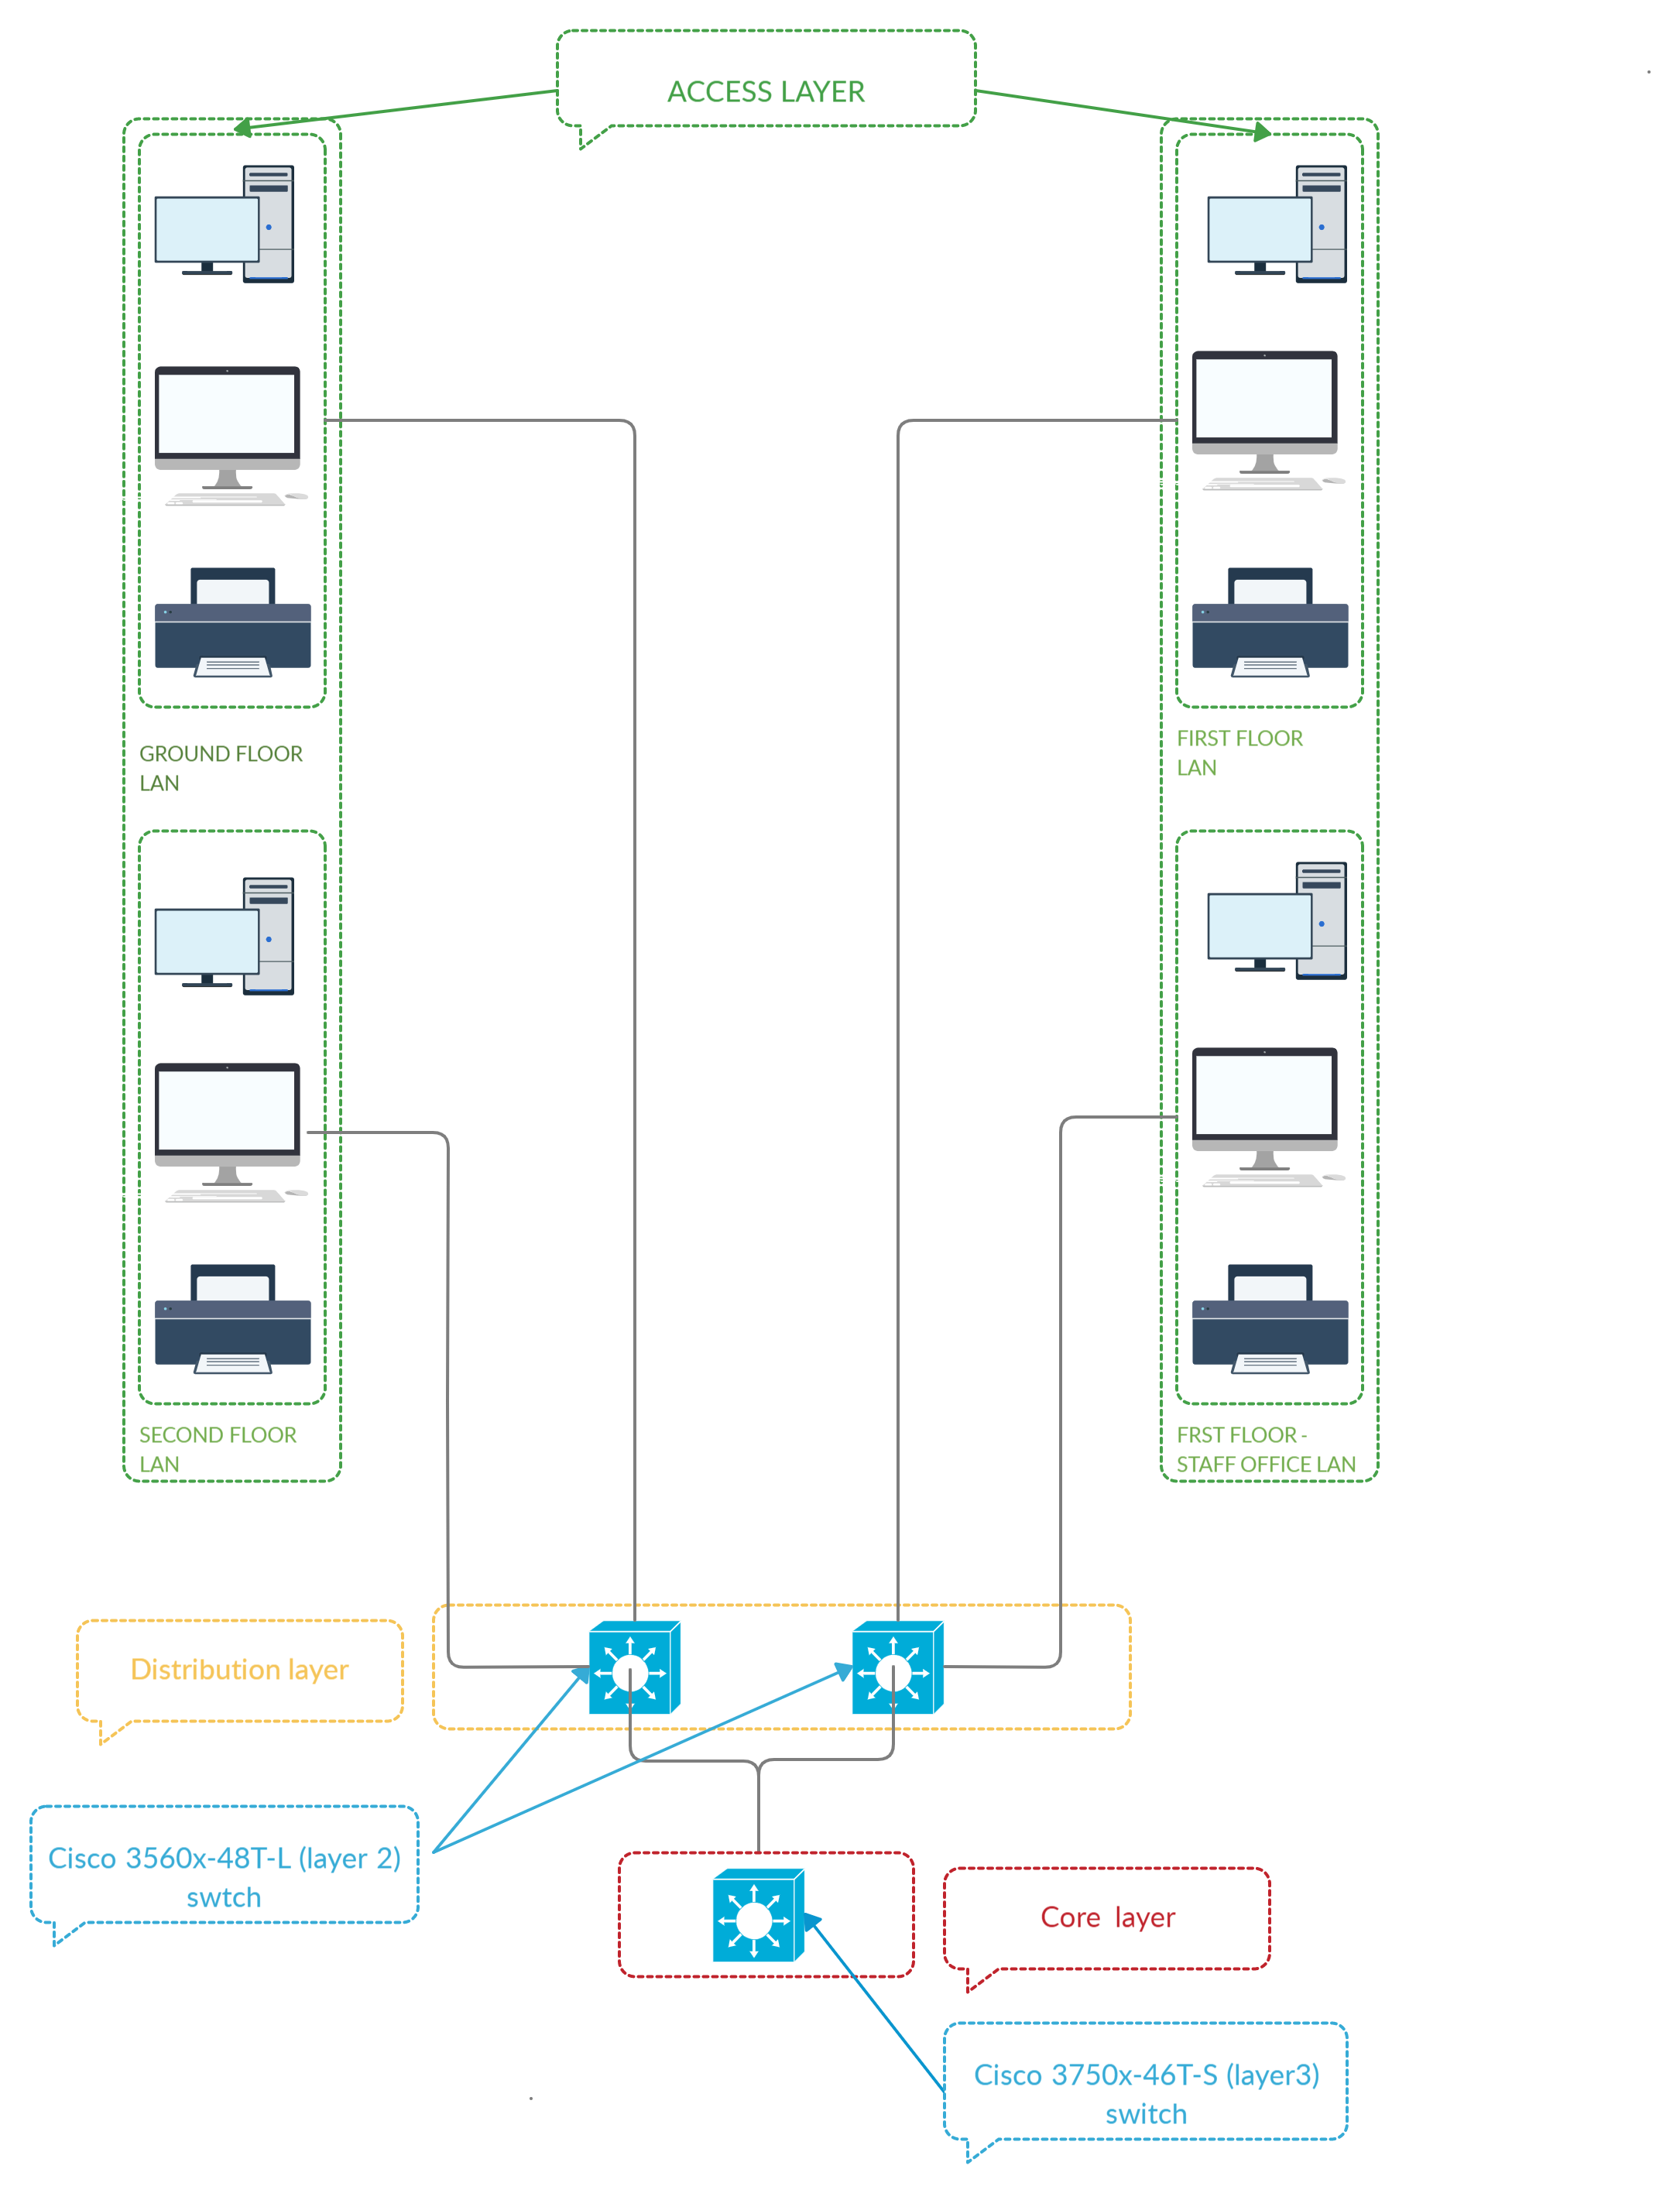
\includegraphics[width=\textwidth]{hnet.png}
    \caption{High level overview of EDN}
\label{fig:heirarch}
  \end{subfigure}
  \hfill
  \begin{subfigure}[b]{0.5\textwidth}
    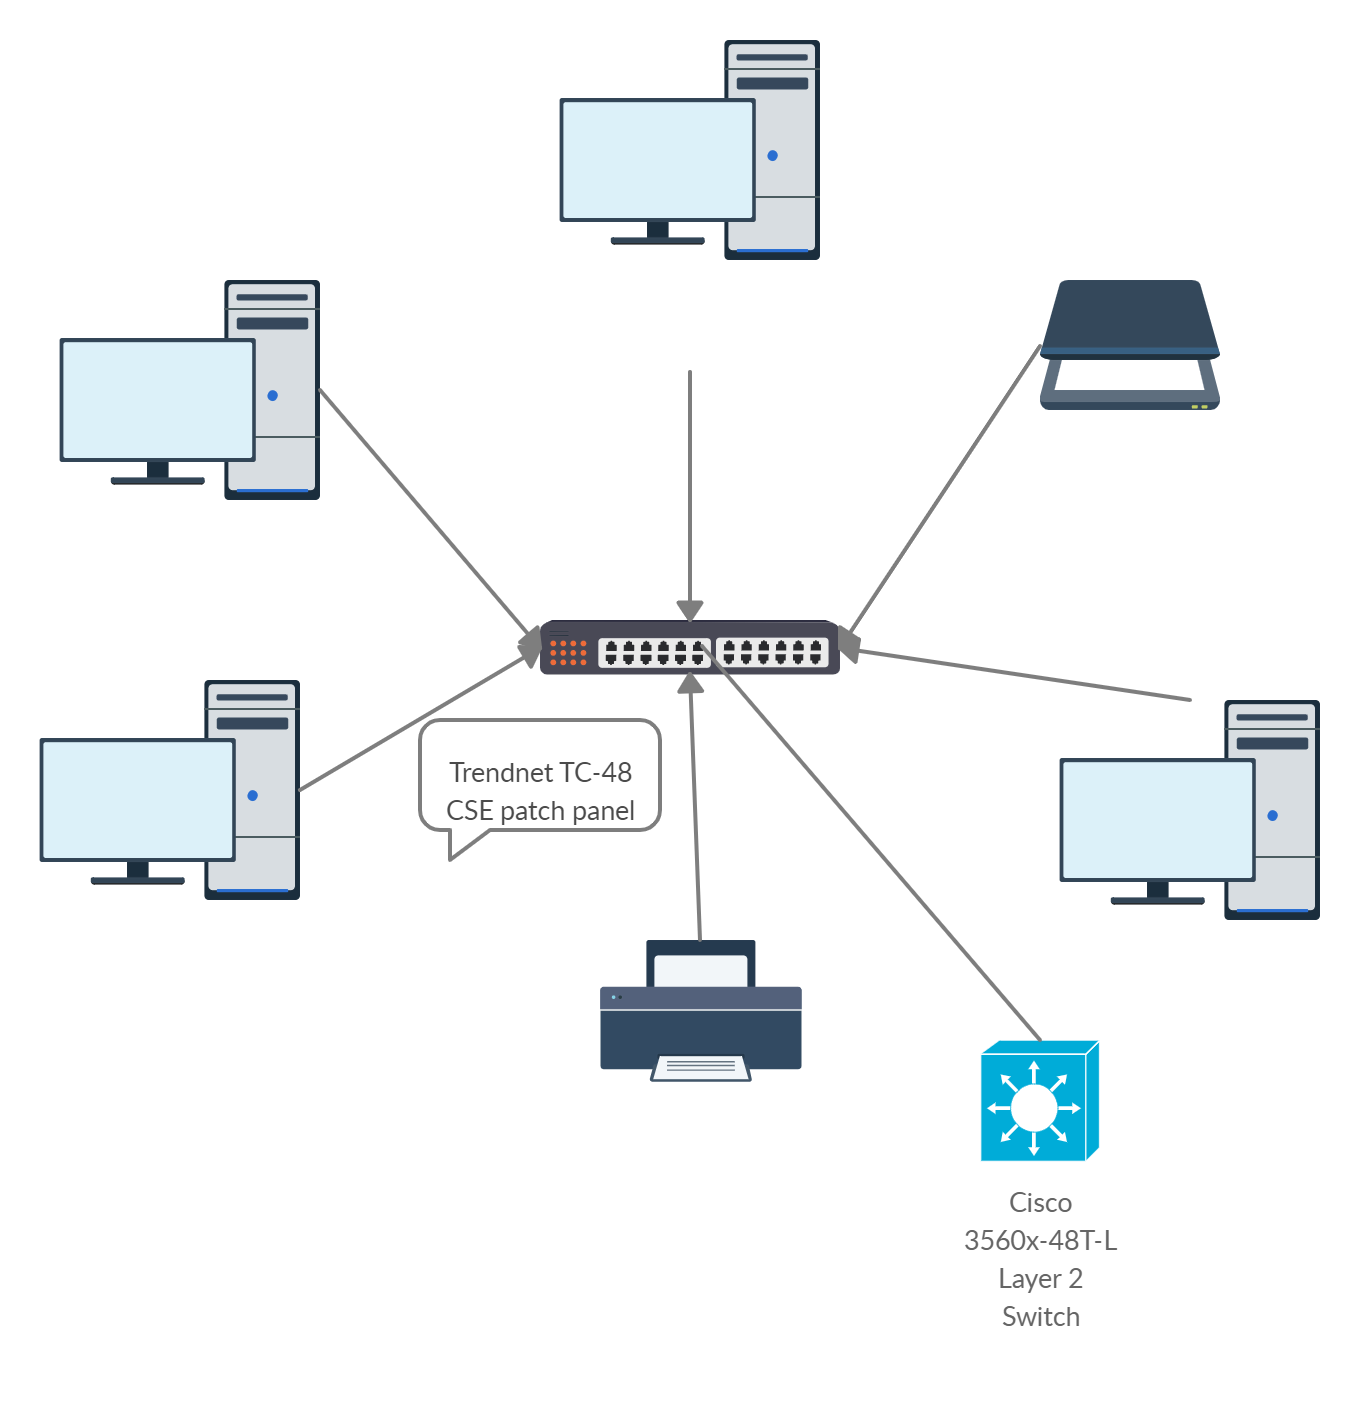
\includegraphics[width=\textwidth]{star.png}
    \caption{EDN Floor LAN configuration}
\label{fig:str}
  \end{subfigure}
  \caption{High level overview of the network and the local area network of each workgroup }
\end{figure}
Finally, \textbf{routing will be handled by the multilayer switches} in the Core and Distribution layers as well as a router which I will refer to as EDGE router.
In this design, I break EDN into VLANs (Virtual Local Area Network), due to the fact that VLANs improve the security of the network, minimize the routers deployed on the network to absorb broadcast traffic and enable logical grouping of end-clients that are physically dispersed on a network. In the distribution layer, EDN will have two multilayer switches which will act as bridges between the access layer and core layer and handle the IP routing between subnets. Ideally we would have one multilayer switch per workgroup, however here we choose only two. EDN can be further scaled when the number of users expands.

\subsection{Internet access}
For internet access we will have the EDGE router connected between the core layer multilayer switch and the ISP provider. The connection to the quad 8 DNS (Domain Name Server) will be simulated and tested in future sections.

\subsection{Network optimization}
EDN will have the HSRP standard (Hot Standby Router Protocol) configured, as it routes traffic without relying on the availability of any single router.
To prevent bridge loops and incorporate backup links (to provide fault tolerance if an active link fails) I implemented the STP (Spanning Tree Protocol) set up. Furthermore, EDN will employ the Enhanced Interior Gateway Routing Protocol (EIGRP) which reduces the workload on the router and the amount of data to be propagated. Moreover, EIGRP will allow us to set up connections to the other buildings networks in the university. Additionally, I will also use Network address translation (NAT) to allow routers to modify packets, and for multiple devices to share a single public IP address.

\subsection{Security}
To be physically secured, EUL will handout access cards to its employees so that only authorized individuals have the right to enter the ED building.
For logical security, EDN switches will have port security set up. Then, the router in the network will be accessed via SSH. Finally, the routers, switches and wireless access points in the network will be password protected with a correct banner. \\
\textbf{NB}: Wireless access points will employ WPA2-PSK scheme for password protection in addition to the the Advanced Encryption Standard (AES). 

\subsection{IP addressing}
In this project, EDN was assigned class C 204.15.5.0 network, to be subnetted across the 3 floors with \textbf{a required maximum hosts per subnet of 30	}. Table \ref{tbl:usrs} describes how the number of users is distributed throughout the building. The correct subnet mask for this is then 255.255.255.224 (/27). This subnet mast will divide the network into 8 subnets, with exactly 30 hosts per subnet. We will choose 4 subnets and leave the rest for future use. Three subnets will be assigned to the ground, first and second floor. One subnet will be assigned to the staff office on the first floor. Each subnet in EDN is configured as a VLAN. Table \ref{tbl:subnts} describes how the subnets are assigned to each floor.
Users on the network will be assigned IP addresses dynamically via the DHCP (Dynamic Host Configuration Protocol).
\begin{table}[h!]
\scalebox{1.5}{
\begin{tabular}{l|l|l}
	Floor			& Work group            & No.users    \\\hline
	Ground   			& Administration, staff office, labs, seminar rooms and lecture  theatre & \textbf{30} \\
	1st floor A     			& Laboratories & \textbf{30}  \\
	1st floor B     			& staff office & \textbf{14} \\
	2nd floor     			& Microlabs, staff office, seminar rooms & \textbf{25} \\
\end{tabular}
}
\caption{Distribution of users in each floor of the ED building}
\label{tbl:usrs}
\end{table}

\begin{table}[h!]
\scalebox{1.5}{
\begin{tabular}{l|l|l|l}
	Floor			& VLAN            & Net ID  & Default-gateway  \\\hline
	Ground   			& 1 & \textbf{204.15.5.0} &  \textbf{204.15.5.1} \\
	1st floor A     			& 32 & \textbf{204.15.5.32}&  \textbf{204.15.5.33} \\
	1st floor B     			& 64 & \textbf{204.15.5.64} & \textbf{204.15.5.65} \\
	2nd floor     			& 96 & \textbf{204.15.5.96} & \textbf{204.15.5.97} \\
\end{tabular}
}
\caption{Subnet and VLAN per floor}
\label{tbl:subnts}
\end{table}
\clearpage 
\subsection{OSI model}
Table \ref{tbl:osi} describes the protocols to be used in EDN's OSI layers.

\begin{table}[h!]
\scalebox{1.5}{
\begin{tabular}{l|l}
	Layer			& Protocol              \\\hline
	Application		& HTTP, FTP, SMTP, DHCP, DNS, SSH  \\
	Presentation  			& SSL, ASCII, gzip  \\
	Session    			& NetBios  \\
	Transport     			& TCP, UDP, NAT \\
	Network     			& IP, ICMP \\
	Data link     			& ARP, Ethernet, \textbf{EIGRP},IEEE 802.3, \textbf{IEEE 802.1w} (RSTP)  \\
	Physical     			& 100BASE-TX, 1000BASE-FX \\
\end{tabular}
}
\caption{OSI layers protocols}
\label{tbl:osi}
\end{table} 

\section{Implementation}
\subsection{Network implementation using Cisco Packet Tracer}
In this section we will discuss the details of EDN implementation employing the Cisco Packet Tracer tool.
Figure \ref{fig:pckt} depicts EDN on Packet tracer. Notice that we have not included all the devices in the access layer, due to the fact that only one device is sufficient to demonstrate our design, and that each subnet is configured with the right amount of users with DHCP protocol dynamically assigning IP addresses. The following subsections include the code I employed to configure the whole network, I also added comments when needed. The majority of the code is repeated across devices, therefore I will only demonstrate the code executed on one device correspondingly.

\begin{figure}[H]
\caption{EDN implementation on Cisco Packet tracer}
\begin{center}
  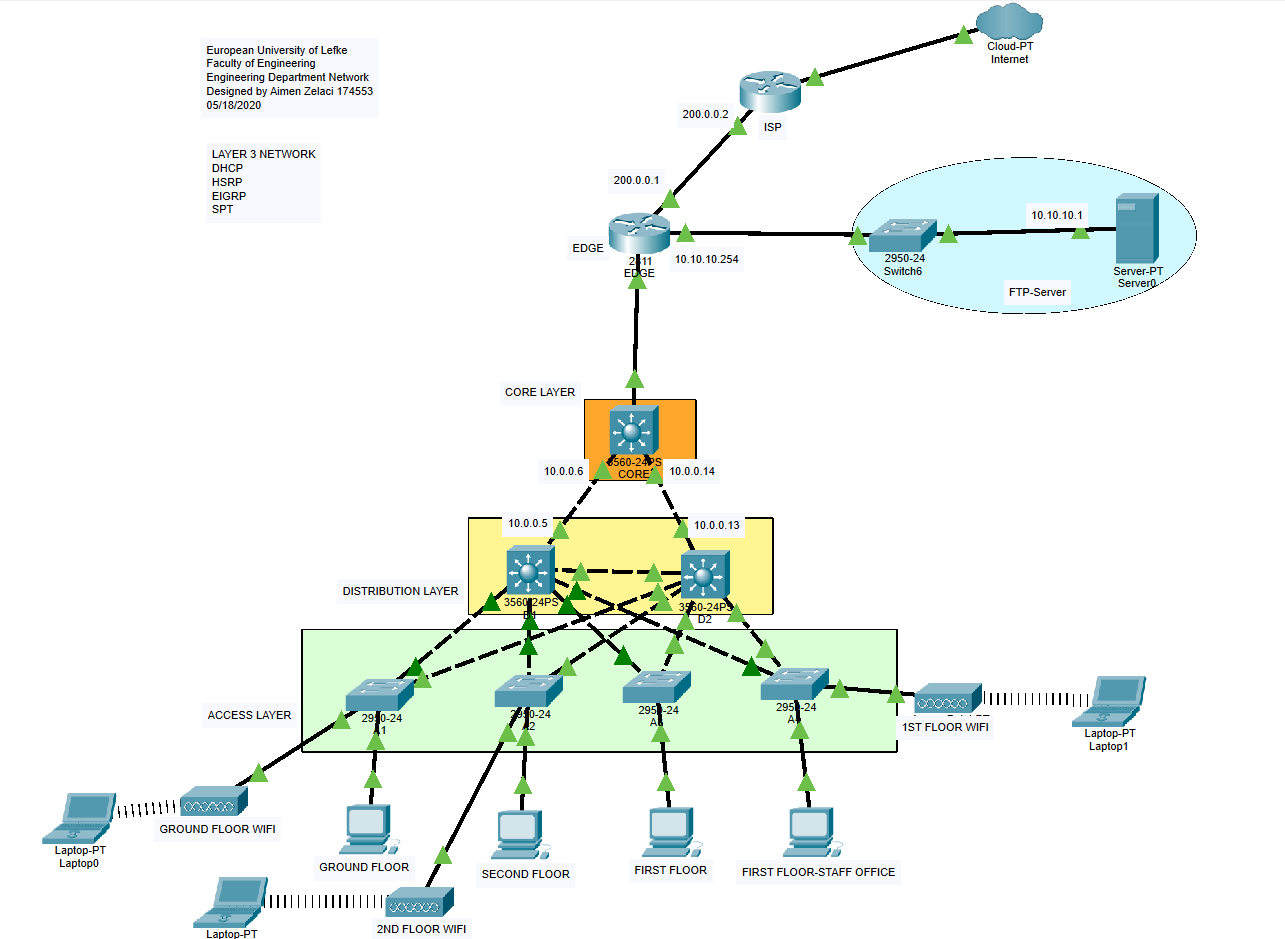
\includegraphics[width=0.95\linewidth]{packett.png}
\end{center}
\label{fig:pckt}
\end{figure}

\subsection{VLAN configuration}
The following code sets up the VLANs in the network. The same code is executed for the other distribution and access layers switches. However, we will have only two VLANs per access layer switch.\\
\textbf{NB}: This code applies to the distribution and access layer, whereas for the core layer I configured interfaces between that layer and the distribution layer, with IP scheme of 10.0.0.0/30.
\begin{center}
\begin{lstlisting}

Switch> enable
Switch# conf t
Switch(conf)# hostname D1
D1(conf)# vlan 1
D1(conf)# vlan 32
D1(conf)# vlan 64
D1(conf)# vlan 96
D1(conf)# ^Z
D1# show vlan
VLAN Name                             Status    Ports
---- -------------------------------- ---------
1    default                          active    Fa0/1, Fa0/2, Fa0/3, Fa0/4
                                                Fa0/5, Fa0/6, Fa0/7, Fa0/8
                                                Fa0/9, Fa0/10, Fa0/11, Fa0/12
                                                Fa0/13, Fa0/14, Fa0/15,Fa0/16
                                                Fa0/17, Fa0/18, Fa0/19,Fa0/20
                                                Gig0/1, Gig0/2
32   VLAN0032                         active    
64   VLAN0064                         active    
96   VLAN0096                         active    
1002 fddi-default                     active    
1003 token-ring-default               active    
1004 fddinet-default                  active    
1005 trnet-default                    active    
D1#wr
Building configuration...
[OK]
D1#
\end{lstlisting}
\end{center}

\subsection{VLAN INTERFACES CONFIGURATION}
The first distribution layer will have a 204.15.5.x ip address whereas the other will have 204.15.5.y , such that $x = \{2, 34, 66, 98\}$ and $y = \{3, 35, 67, 99\}$ .
The same code will be employed for both switches, with those IP addresses differences taken into account. 
\begin{center}
\begin{lstlisting}

D1> enable
D1# conf t
D1(conf)# int vlan 1
D1(conf-if)# ip add 204.15.5.2 255.255.255.224
D1(conf-if)# ex
D1(conf)# int vlan 32
D1(conf-if)# ip add 204.15.5.34 255.255.255.224
D1(conf-if)# ex
D1(conf)# int vlan 64
D1(conf-if)# ip add 204.15.5.66 255.255.255.224
D1(conf-if)# ex
D1(conf)# int vlan 96
D1(conf-if)# ip add 204.15.5.98 255.255.255.224
D1(conf-if)# ex
D1(conf)#^Z
D1#sh ip int br | ex un
Interface              IP-Address      OK? Method Status                Protocol 
Vlan1                  204.15.5.2      YES manual up                    up 
Vlan32                 204.15.5.34     YES manual up                    up 
Vlan64                 204.15.5.66     YES manual up                    up 
Vlan96                 204.15.5.98     YES manual up                    up
D1#

\end{lstlisting}
\end{center}

\subsection{DHCP CONFIGURATION}
First, we exclude the IP addresses used as interfaces for our multilayer switches as well as the default gateways. Then, we assign the correct DHCP pool for the clients.
\begin{center}
\begin{lstlisting}

D1> enable
D1# conf t
D1(conf)# ip dhcp exclude 204.15.5.1 204.15.5.3
D1(conf)# ip dhcp exclude 204.15.5.33 204.15.5.35
D1(conf)# ip dhcp exclude 204.15.5.65 204.15.5.67
D1(conf)# ip dhcp exclude 204.15.5.97 204.15.5.99
D1(conf)# ip dhcp pool vlan1
D1(dhcp-conf)# net 204.15.5.0 255.255.255.224
D1(dhcp-conf)# defau 204.15.5.1
D1(dhcp-conf)# domain google.com
D1(dhcp-conf)# dns 8.8.8.8
D1(dhcp-conf)# ex
D1(conf)# ip dhcp pool vlan32
D1(dhcp-conf)# net 204.15.5.32 255.255.255.224
D1(dhcp-conf)# defau 204.15.5.33
D1(dhcp-conf)# domain google.com
D1(dhcp-conf)# dns 8.8.8.8
D1(dhcp-conf)# ex
D1(conf)# ip dhcp pool vlan64
D1(dhcp-conf)# net 204.15.5.64 255.255.255.224
D1(dhcp-conf)# defau 204.15.5.65
D1(dhcp-conf)# domain google.com
D1(dhcp-conf)# dns 8.8.8.8
D1(dhcp-conf)# ex
D1(conf)# ip dhcp pool vlan96
D1(dhcp-conf)# net 204.15.5.96 255.255.255.224
D1(dhcp-conf)# defau 204.15.5.97
D1(dhcp-conf)# domain google.com
D1(dhcp-conf)# dns 8.8.8.8
D1(dhcp-conf)# ex
D1(conf)#
\end{lstlisting}
\end{center}
\subsection{HSRP CONFIGURATION}
We will set the first multilayer switch (D1) in the distribution layer to act as a primary router for VLAN 1 and 96 and secondary for VLAN 32 and 64. Whereas the second switch (D2) will act vice versa.
The following code is executed on the D1 distribution layer. At the end of the code you may see that everything is configured correctly.
\begin{center}
\begin{lstlisting}

D1> enable
D1# conf t
D1(conf)# int vlan 1
D1(conf-if)# standby 1 ip 204.15.5.1
D1(conf-if)# standby 1 prio 120
D1(conf-if)# standby 1 pre
D1(conf-if)#ex
D1(conf)# int vlan 96
D1(conf-if)# standby 96 ip 204.15.5.97
D1(conf-if)# standby 96 prio 120
D1(conf-if)# standby 96 pre
D1(conf-if)#ex
D1(conf)# int vlan 32
D1(conf-if)# standby 32 ip 204.15.5.33
D1(conf-if)#ex
D1(conf)# int vlan 64
D1(conf-if)# standby 64 ip 204.15.5.65
D1(conf-if)#ex
D1(conf)#^Z
D1#sh stan br
                     P indicates configured to preempt.
                     |
Interface   Grp  Pri P State    Active          Standby         Virtual IP
Vl1         1    120 P Active   local           204.15.5.3      204.15.5.1     
Vl32        32   100   Standby  204.15.5.35     local           204.15.5.33    
Vl64        64   100   Standby  204.15.5.67     local           204.15.5.65    
Vl96        96   120 P Active   local           204.15.5.99     204.15.5.97    
D1#

\end{lstlisting}
\end{center}
\subsection{Trunking}
The following, is the code executed on switch D1 (distribution layer) to truncate the lines between switches (lines that handle the traffic). At the end of the code you may see that everything is configured correctly. This code will be executed for all switches in the network.
\begin{center}
\begin{lstlisting}

D1> enable
D1#conf t
D1(conf)# int gig0/1
D1(config-if)#switchport trunk encapsulation dot1q 
D1(config-if)#switchport mode trunk
D1(config-if)#switchport nonnegociate
D1(conf-if)# ex
D1(conf)# int ra fa0/19 - 24
D1(config-if)#switchport trunk encapsulation dot1q 
D1(config-if)#switchport mode trunk
D1(config-if)#switchport nonnegociate
D1(conf-if)# ex
D1(conf)#^Z
D1#sh cdp n
Capability Codes: R - Router, T - Trans Bridge, B - Source Route Bridge
                  S - Switch, H - Host, I - IGMP, r - Repeater, P - Phone
Device ID    Local Intrfce   Holdtme    Capability   Platform    Port ID
A3           Fas 0/24         167            S       2950        Fas 0/24
CORE         Fas 0/20         167                    3560        Fas 0/23
A2           Fas 0/23         167            S       2950        Fas 0/24
A1           Fas 0/21         167            S       2950        Fas 0/23
A4           Fas 0/22         167            S       2950        Fas 0/24
D2           Gig 0/1          175                    3560        Gig 0/1
D1#
\end{lstlisting}
\end{center}
\subsection{HSRP - Synchronization of primary routers with the bridge}
Switch D1 will be the primary route for vlan 1, 96 as shown here:
\begin{center}
\begin{lstlisting}

D1>en
D1#sh stan br
                     P indicates configured to preempt.
                     |
Interface   Grp  Pri P State    Active          Standby         Virtual IP
Vl1         1    120 P Active   local           204.15.5.3      204.15.5.1     
Vl32        32   100   Standby  204.15.5.35     local           204.15.5.33    
Vl64        64   100   Standby  204.15.5.67     local           204.15.5.65    
Vl96        96   120 P Active   local           204.15.5.99     204.15.5.97    
D1#
\end{lstlisting}
\end{center}
For switch D2 this will be the exact opposite:
\begin{center}
\begin{lstlisting}

D2>en
D2#sh stan br
                     P indicates configured to preempt.
                     |
Interface   Grp  Pri P State    Active          Standby         Virtual IP
Vl1         1    100   Standby  204.15.5.2      local           204.15.5.1     
Vl32        32   120 P Active   local           204.15.5.34     204.15.5.33    
Vl64        64   120 P Active   local           204.15.5.66     204.15.5.65    
Vl96        96   100   Standby  204.15.5.98     local           204.15.5.97    
D2#
\end{lstlisting}
\end{center}
We will now match them with the correct spanning tree (in the following subsection).
\subsection{Spanning-Tree configuration}
For D1:
\begin{center}
\begin{lstlisting}

D1>en    
D1#conf t
D1(conf)# spanning-tree vlan 1,96 root primary
D1(conf)# spanning-tree vlan 32,64 root secondary
\end{lstlisting}
\end{center}
For D2:
\begin{center}
\begin{lstlisting}

D2>en    
D2#conf t
D2(conf)# spanning-tree vlan 32,64 root primary
D2(conf)# spanning-tree vlan 1,96 root secondary
\end{lstlisting}
\end{center}
Next, we enable rapid PVST+ for all the switches in the network (see \ref{sec:bib} for more information):
\begin{center}
\begin{lstlisting}

D1>en    
D1#conf t
D1(conf)# spann mode rapid
\end{lstlisting}
\end{center}
\subsection{Access layer port configuration}
In this subsection we demonstrate how ports of the switches in the Access layer are assigned to their corresponding VLAN. The code is similar for all the switches, the following is for the first switch in the access layer (A1):
\begin{center}
\begin{lstlisting}

A1>en    
A1#conf t
A1(conf)# int ra fa 0/1 - 22
A1(conf-if)# switchport mode access 
A1(conf-if)# switchport access vlan 1
A1(conf-if)# spanning-tree port-fast
A1(conf-if)# spanning-tree bpqguard enable
A1(conf-if)# switchport nonnegociate
A1(conf-if)# storm-control broadcast level 40
\end{lstlisting}
\end{center}
\textbf{NB}: The storm control enables the device to monitor traffic levels and to drop broadcast. 
\subsection{Switch port security}
As the following code demonstrates, no more than 2 devices with different mac addresses can be connected to the same port. Therefore, if an intruder plugs his device in EDN the port will shut down and EDN administrators will be alerted.

\begin{center}
\begin{lstlisting}

A1>en    
A1#conf t
A1(conf)# int ra fa 0/1 - 22
A1(conf-if)# switchport port-security mac-address sticky
A1(conf-if)# switchport port-security maximum 2
A1(conf-if)# switchport port-security violation restrict 
\end{lstlisting}
\end{center}

\subsection{EIGRP}
Switches in the distribution and the core layer, as well as our EDGE router, will be assigned adjacency by configuring the EIRGP, as the following code demonstrates:
\begin{center}
\begin{lstlisting}


CORE # do show route connected
CORE(config)#do sh ip rou con
 C   10.0.0.4/30  is directly connected, FastEthernet0/1
 C   10.0.0.12/30  is directly connected, FastEthernet0/2
 C   10.0.0.56/30  is directly connected, FastEthernet0/24
CORE(conf)# router eigrp 1
CORE(conf-router)# no auto-summary
CORE(conf-router)# net 10.0.0.4 0.0.0.3
CORE(conf-router)# net 10.0.0.12 0.0.0.3
CORE(conf-router)# net 10.0.0.56 0.0.0.3
\end{lstlisting}
\end{center}

 \subsection{Router configuration}
 The following code configures our EDGE router interfaces as well as the EIRGP adjacency.
\begin{center}
\begin{lstlisting}


Router > en
Router # conf t
Router(conf)# host EDGE
EDGE(conf)# int fastEthernet 0/0
EDGE(conf-if)# ip add 200.0.0.1 255.255.255.252
EDGE(conf-if)# no shutdown
EDGE(conf-if)# ip route 0.0.0.0 0.0.0.0 fastEthernet 0/0
EDGE(config)#do show ip route connected
 C   10.0.0.56/30  is directly connected, FastEthernet0/1
 C   10.10.10.0/24  is directly connected, FastEthernet1/0
 C   200.0.0.0/30  is directly connected, FastEthernet0/0
EDGE(config)# router eigrp 1
EDGE(config-router)# no auto-summary
EDGE(config-router)# net 10.0.0.56 0.0.0.3
EDGE(config-router)# redistribute static
EDGE(config-router)# ex
EDGE(config)# ip access-list standard EDNAT
EDGE(config-std-nacl)# permit any
EDGE(config-std-nacl)# ex
EDGE(config)# ip nat inside source list EDNAT interface fastEthernet 0/0 overload 
EDGE(config)# int fa0/1
EDGE(config-if)# ip nat in
EDGE(config-if)# ex
EDGE(config)# int fa0/0
EDGE(config-if)# ip nat out

\end{lstlisting}
\end{center}
NB: Please note that NAT is configured in the above code as well.
Now that everything is configured correctly, we may see the routing table set up:

\begin{center}
\begin{lstlisting}


CORE#sh ip route
Codes: C - connected, S - static, I - IGRP, R - RIP, M - mobile, B - BGP
       D - EIGRP, EX - EIGRP external, O - OSPF, IA - OSPF inter area
       N1 - OSPF NSSA external type 1, N2 - OSPF NSSA external type 2
       E1 - OSPF external type 1, E2 - OSPF external type 2, E - EGP
       i - IS-IS, L1 - IS-IS level-1, L2 - IS-IS level-2, ia - IS-IS inter area
       * - candidate default, U - per-user static route, o - ODR
       P - periodic downloaded static route

Gateway of last resort is 10.0.0.57 to network 0.0.0.0

     10.0.0.0/30 is subnetted, 3 subnets
C       10.0.0.4 is directly connected, FastEthernet0/1
C       10.0.0.12 is directly connected, FastEthernet0/2
C       10.0.0.56 is directly connected, FastEthernet0/24
     204.15.5.0/27 is subnetted, 4 subnets
D       204.15.5.0 [90/25628160] via 10.0.0.13, 01:38:44, FastEthernet0/2
                   [90/25628160] via 10.0.0.5, 01:38:44, FastEthernet0/1
D       204.15.5.32 [90/25628160] via 10.0.0.13, 01:38:44, FastEthernet0/2
                    [90/25628160] via 10.0.0.5, 01:38:44, FastEthernet0/1
D       204.15.5.64 [90/25628160] via 10.0.0.13, 01:38:44, FastEthernet0/2
                    [90/25628160] via 10.0.0.5, 01:38:44, FastEthernet0/1
D       204.15.5.96 [90/25628160] via 10.0.0.13, 01:38:44, FastEthernet0/2
                    [90/25628160] via 10.0.0.5, 01:38:44, FastEthernet0/1
D*EX 0.0.0.0/0 [170/53760] via 10.0.0.57, 01:38:45, FastEthernet0/24

CORE #
\end{lstlisting}
\end{center}
 
 \subsection{Authorization}
To avoid dictionary attacks we will first set the password length on our router and switch to a minimum of 8. Next, we set an admin user with the highest privilege rights of 15. Then we set a timeout of 1 minute. Finally, we set up a banner "FOR AUTHORIZED USERS BY EUL MANAGEMENT ONLY" and enable SSH access to the EDGE router.
\begin{center}
\begin{lstlisting}


EDGE #conf t

EDGE(conf)# security password min-length 8
EDGE(conf)# line console 0
EDGE(conf-line)#  username EDadmin preivilege 15 secret eul199000 
EDGE(conf-line)# login local
EDGE(conf-line)# exec-timeout 1 00
EDGE(conf)# login block-for 300 attempts 3 within 30
EDGE(conf)# banner motd & FOR AUTHORIZED USERS BY EUL MANAGEMENT ONLY
EDGE(conf)# ip domain-name EDN
EDGE(conf)# crypto key generate rsa
The name for the keys will be: EDGE.EDN
Choose the size of the key modulus in the range of 360 to 2048 for your
  General Purpose Keys. Choosing a key modulus greater than 512 may take
  a few minutes.

How many bits in the modulus [512]: 2048
% Generating 2048 bit RSA keys, keys will be non-exportable...[OK]
EDGE(conf)#
*Mar 1 1:58:51.966: %SSH-5-ENABLED: SSH 1.99 has been enabled
EDGE(conf)#line vty 0 4
EDGE(conf-line)# transport input ssh
EDGE(conf-line)#

\end{lstlisting}
\end{center} 

\section{Results and Discussion}
In this section we will test our implementation which was discussed in detail in the previous sections. 
First, we will check if the users in the inter VLANS can communicate.
As you can see in figure \ref{fig:test1}, we are able to ping from one end in a LAN to another in a different LAN successfully.
\begin{figure}[H]
  \begin{subfigure}[b]{0.4\textwidth}
    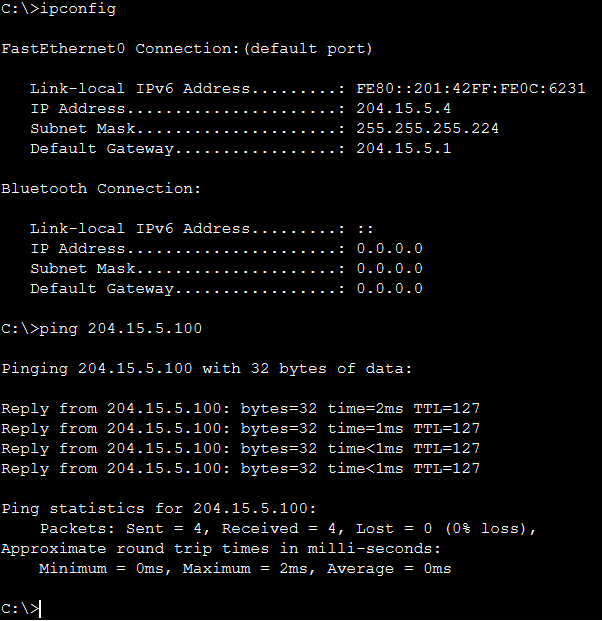
\includegraphics[width=\textwidth]{comm.png}
    \caption{ping from Ground floor to the second floor}
  \end{subfigure}
  \hfill
  \begin{subfigure}[b]{0.4\textwidth}
    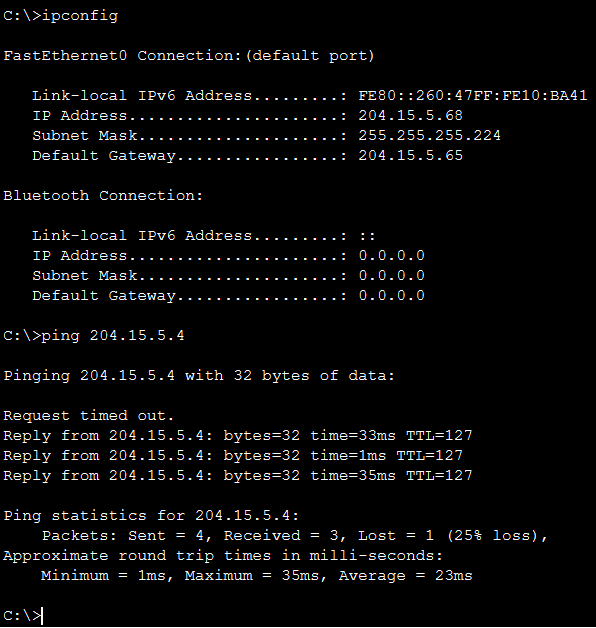
\includegraphics[width=\textwidth]{comm2.png}
    \caption{ping from the first floor to the ground floor}
  \end{subfigure}
  \caption{Local communication test}
  \label{fig:test1}
\end{figure}
Next, we test the SSH that we set up:
\begin{figure}[H]
    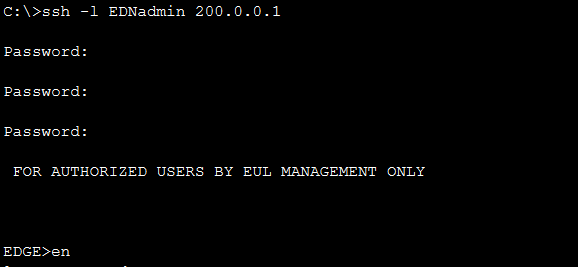
\includegraphics[width=0.5\textwidth]{ssh.png}
    \caption{SSH access}
    \label{fig:test2}
\end{figure}
As you can see our EDGE router is securely accessed via SSH.
	
Finally, I tested the EDN connection to the internet and to the FTP server. Figure \ref{fig:test3} depicts the successful ping to the quad 8 DNS we set up earlier (google's DNS). Figure \ref{fig:test4} shows that an FTP connection has been established correctly. I also tested the internet access via the browser and depicts the result in Figure \ref{fig:test5} 

\begin{figure}[H]
  \begin{subfigure}[b]{0.4\textwidth}
    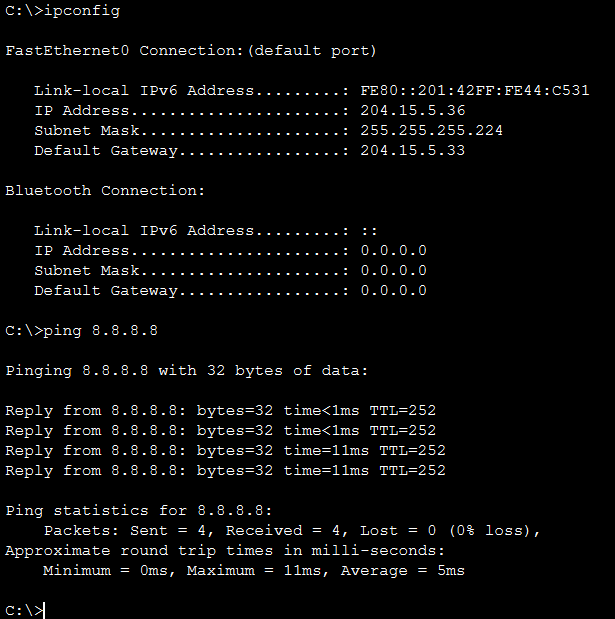
\includegraphics[width=\textwidth]{internet.png}
    \caption{Internet access}
\label{fig:test3}  
  \end{subfigure}
  \hfill
  \begin{subfigure}[b]{0.4\textwidth}
    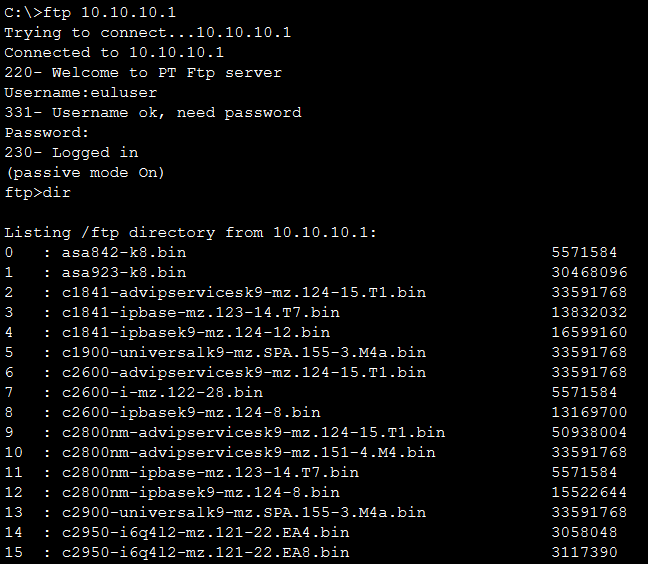
\includegraphics[width=\textwidth]{ftp.png}
    \caption{FTP access}
\label{fig:test4}  
  \end{subfigure}
  \caption{Internet and FTP simulation results}
\end{figure}

\begin{figure}[H]
\centering
    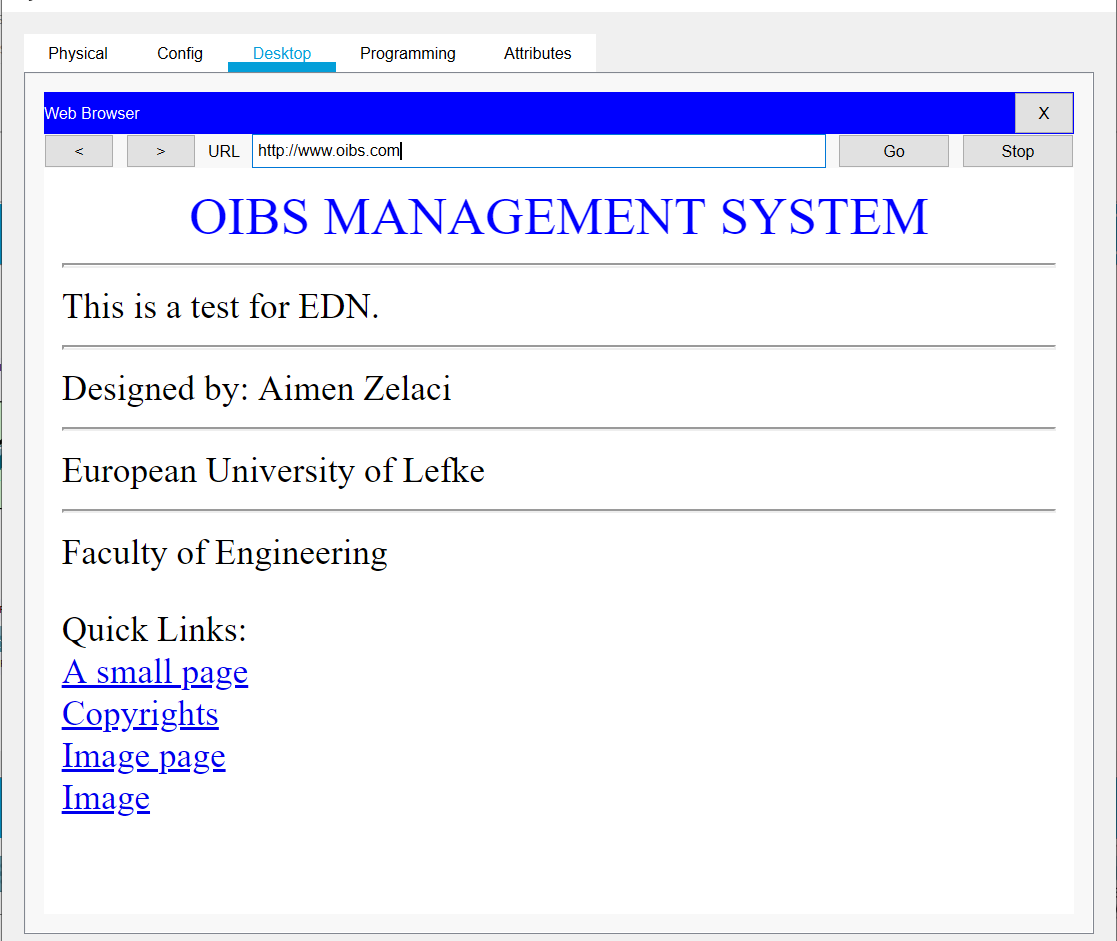
\includegraphics[width=0.6\textwidth]{oibs.png}
    \caption{Oibs management system access test}
    \label{fig:test5}
\end{figure}

\section{Conclusion}
In this project design, I propose the implementation of the Engineering Department building Network. I chose a hierarchical approach for the network to meet the requirements imposed, namely security, interactivity, reliability, and adaptability. I subnetted the network into four Local Area Networks whereby each LAN takes the start topology. I employed several up to date protocols to optimize the network. Moreover, I implemented the latest security schemes. The simulation results on the Cisco Packet tracer show that the network proposed provides the services desired (HTTP, FTP, among others) function efficiently. This design allow EDN for future scale and access to the Wide Area Network of the entire university.
\section{Bibliography}
\label{sec:bib}
\begin{itemize}
\item Introducing Network Design Concepts CCNA. Chapter I. pages 1-5. \url{http://students.mimuw.edu.pl/~zbyszek/sieci/CCNA4%20Sample.pdf}

\item Michael J. Smith, ITN 100. Accounting and Financial Services Corp. Network Design Proposal, November 14, 2011. \url{http://mikejsmith.net/wp-content/uploads/2013/01/Sample_Network_Design.pdf}

\item Botsford, Charles. “Learn To Subnet.com v. 3.2.” LearnTCPIP.com. N. p., n. d. Web. 3 November 2011. \url{http://www.learntcpip.com/LTSN/default.htmNoember 2011}
\item Campus network design 

\item “Network Design for Small Business.” BeginLinux.com. N.p. 3 June 2010. N. pag. Web. 3 November 2011. \url{http://beginlinux.com/blog/2010/06/network-design-for-a-small-business}

\item Chapter: Configuring Rapid PVST+, Cisco Nexus 5000 Series NX-OS Software Configuration Guide. \url{cisco.com/c/en/us/td/docs/switches/datacenter/nexus5000/sw/configuration/guide/cli/CLIConfigurationGuide/RPVSpanningTree.html}

\item Enhanced Interior Gateway Routing Protocol, Wikipedia. \url{https://en.wikipedia.org/wiki/Enhanced_Interior_Gateway_Routing_Protocol}

\item Network address translation, Wikipedia. \url{https://en.wikipedia.org/wiki/Network_address_translation}
\end{itemize}	

\end{document}